% Created 2019-05-19 Sun 23:31
% Intended LaTeX compiler: pdflatex
\documentclass[presentation]{beamer}
\usepackage[utf8]{inputenc}
\usepackage[T1]{fontenc}
\usepackage{graphicx}
\usepackage{grffile}
\usepackage{longtable}
\usepackage{wrapfig}
\usepackage{rotating}
\usepackage[normalem]{ulem}
\usepackage{amsmath}
\usepackage{textcomp}
\usepackage{amssymb}
\usepackage{capt-of}
\usepackage{hyperref}
\usepackage{awesomebox}
\usepackage{booktabs}
\usepackage{placeins}
\usepackage{siunitx}
\usepackage{minted}
\usetheme[progressbar=frametitle]{metropolis}
\usepackage{tikz}
\usepackage{tikz-3dplot}
\usepackage{spot}
\usepackage{pgfplots}
\usetikzlibrary{arrows.meta}
\pgfplotsset{compat=1.16}
\newcommand{\gv}[1]{\ensuremath{\mbox{\boldmath$ #1 $}}}
\newcommand{\bv}[1]{\ensuremath{\mathbf{#1}}}
\newcommand{\norm}[1]{\left\lVert#1\right\rVert}
\newcommand{\abs}[1]{\left\lvert#1\right\rvert}
\newcommand{\bigqm}[1][1]{\text{\larger[#1]{\text{?}}}}
\newcommand{\order}[1]{\mathcal O \left( #1 \right)} % order of magnitude
\definecolor{scarlet}{rgb}{1.0, 0.13, 0.0}
\definecolor{shamrockgreen}{rgb}{0.0, 0.62, 0.38}
\definecolor{royalblue}{rgb}{0.25, 0.41, 0.88}
\definecolor{metropolisorange}{RGB}{235,129,27}
\definecolor{metropolisblue}{RGB}{35,55,59}
\usetheme{default}
\author{\emph{Tejaswin Parthasarathy}, Mattia Gazzola}
\date{\today}
\title{Elastica : Coordinate/Frame transformations}
\subtitle{ME498: Comp. modeling \& optimization}
\hypersetup{
 pdfauthor={\emph{Tejaswin Parthasarathy}, Mattia Gazzola},
 pdftitle={Elastica : Coordinate/Frame transformations},
 pdfkeywords={},
 pdfsubject={},
 pdfcreator={Emacs 27.0.50 (Org mode 9.2)},
 pdflang={English}}
\begin{document}

\maketitle
\tikzset{>=latex}

\section{Coordinate/Frame transformations}
\label{sec:org0887b34}
\begin{frame}[label={sec:org5fbe9ac}]{Motivation}
\[ \gv{x}_{\mathcal{L}} = \bv{Q}\gv{x} \]
\[ \scalebox{5}{\textbf{?}} \]
\[ \frac{\partial \bv{d}_j}{\partial t} = \left( \bv{Q}^T
   \omega_{\mathcal{L}}\right) \times \bv{d}_j \]
\[ \scalebox{5}{\textbf{?}} \]
\end{frame}

\begin{frame}[label={sec:orgdc88359}]{Motivation}
\begin{columns}
\begin{column}{0.7\columnwidth}
\begin{itemize}
\item To convert between arbitrary spaces, e.g. world space and other spaces (in
graphics) or Eulerian frame to Lagrangian frame in physics
\item To convert between coordinates that are more ``natural'' to the system under
observation---e.g. complex numbers can be naturally represented in polar,
rather than cartesian coordinates
\end{itemize}
\begin{itemize}
\item Transformations can be applied to points, vectors etc.
\end{itemize}
\end{column}
\begin{column}{0.5\columnwidth}
\begin{center}
	\begin{tikzpicture}
	\begin{axis}[
		width=1\textwidth,
		height=0.8\textheight,
		xmin=-1.5,
		xmax=4.5,
		ymin=-4.5,
		ymax=4.5,
		axis equal,
		axis lines=middle,
		grid=major,
		xlabel=$\Re(z)$,
		ylabel=$\Im(z)$,
		disabledatascaling]
		% https://tex.stackexchange.com/questions/27279/how-to-make-an-arrow-bigger-and-change-its-color-in-tikz/27287#27287
		\addplot [arrows={-latex[scale=4]}, thick, color=metropolisorange] coordinates { (0,0) (2,3) } node [right] {$2 + 3i$};
		\addplot [arrows={-latex[scale=4]}, thick, color=metropolisblue] coordinates { (0,0) (3,-2) } node [below] {$3 - 2i$};
		\addplot [black, mark = *] coordinates {( 1, -3)} node [below] {$1 - 3i$};
	\end{axis}
	\end{tikzpicture}
\end{center}
\end{column}

\begin{column}{0.4\columnwidth}
\begin{block}{Cartesian coordinates}
\begin{itemize}
\item Coordinate: \((x, y, z)\)
\item Frame : \(\hat{\gv{e}_x}, \hat{\gv{e}_y}, \hat{\gv{e}_z}\)
\end{itemize}
\end{block}
\end{column}
\begin{column}{0.6\columnwidth}
\begin{figure}[htbp]
\centering
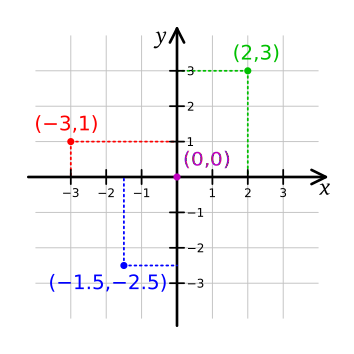
\includegraphics[width=0.8\textwidth]{images/cartesian.pdf}
\caption{Cartesian coordinate system, Wikimedia}
\end{figure}
\end{column}
\end{columns}
\end{frame}
\begin{frame}[label={sec:orgc1c9fb0}]{Introduction}
\begin{columns}
\begin{column}{0.4\columnwidth}
\begin{block}{Cylindrical coordinates}
\begin{itemize}
\item Coordinate: \((\rho, \phi, z)\)
\item Frame : \(\hat{\gv{e}_\rho}, \hat{\gv{e}_\phi}, \hat{\gv{e}_z}\)
\end{itemize}
\tdplotsetmaincoords{60}{110}
\begin{tikzpicture}[tdplot_main_coords, scale=2.8]
	\tikzstyle{every node}=[font=\small]
	\draw[thick,-latex] (0,0,0) -- (1,0,0) node[anchor=north east]{$x$};
	\draw[thick,-latex] (0,0,0) -- (0,1,0) node[anchor=north west]{$y$};
	\draw[thick,-latex] (0,0,0) -- (0,0,1) node[anchor=south]{$z$};
	\draw [thick](0,0,0) circle (0.5);
	\draw [thick](0,0,0.8) circle (0.5);
	\draw [thick](0.22,-0.45,0) -- (0.22,-0.45,0.8) node[midway, left]{$\rho=\rho_1$};
	\draw [thick](-0.22,0.45,0) -- (-0.22,0.45,0.8);
	\filldraw[fill=metropolisorange, nearly transparent] (-0.6,-0.6,0.8) -- (0.6,-0.6,0.8) --  (0.6,0.6,0.8) -- (-0.6,0.6,0.8) -- (-0.6,-0.6,0.8);
	\filldraw[fill=blue, nearly transparent] (0,0,0.8) -- (0.45,0.6,0.8) --  (0.45,0.6,0) -- (0,0,0) -- (0,0,0.8);
	\filldraw [color=metropolisblue](0.3,0.4,0.8) circle (0.03) ;
	\draw (-0.6,0.6,0.8) node[anchor=south]{$z=z_1$};
	\draw (0.6,0.8,0) node[anchor=south west]{$\phi=\phi_1$};
	\draw (-0.1,0.6,0.8) node[above right] { $(\rho_1,\phi_1,z_1)$};
	\draw[thick,-latex](0.3,0.4,0.8) -- (0.48,0.64,0.8) node[anchor=north] {$\hat{\gv{e}_\rho}$};
	\draw[thick,-latex](0.3,0.4,0.8) -- (0.12,0.52,0.8) node[anchor=north west]{$\hat{\gv{e}_\phi}$};
	\draw[thick,-latex](0.3,0.4,0.8) -- (0.3,0.4,1.1) node[anchor=north west]{$\hat{\gv{e}_z}$};
	\draw [thick,->](0.8,0,0) arc (0:53.14:0.8);
	% \draw (0.8,0.3,0) node[anchor=north] {$\phi_1$};
	\draw[thick,-latex,metropolisblue](0,0,0) -- (0.3,0.4,0);
	\draw (0.20,0.12,0) node[anchor=north] {$\rho_1$};
	\draw [thick,metropolisblue,-latex] (0.3,0.4,0)--(0.3,0.4,0.8);
	%\draw[ultra thick](0.1,0,4) -- (-0.1,0,4) node[anchor=south west] {$z_1$};
\end{tikzpicture}
\end{block}
\end{column}

\begin{column}{0.4\columnwidth}
\begin{block}{Spherical coordinates}
\begin{itemize}
\item Coordinate: \((r, \theta, \phi)\)
\item Frame : \(\hat{\gv{e}_r}, \hat{\gv{e}_\theta}, \hat{\gv{e}_\phi}\)
\end{itemize}

% 3D axis with spherical coordinates
\tdplotsetmaincoords{60}{110}
\begin{tikzpicture}[scale=3,tdplot_main_coords]

	% variables
	\def\rvec{1.2}
	\def\thetavec{40}
	\def\phivec{60}

	\def\rvecplus{0.3}
	\def\thetavecplus{8}
	\def\phivecplus{15}
	% axes
	\coordinate (O) at (0,0,0);
	\draw[thick,->] (0,0,0) -- (1,0,0) node[anchor=north east]{$x$};
	\draw[thick,->] (0,0,0) -- (0,1,0) node[anchor=north west]{$y$};
	\draw[thick,->] (0,0,0) -- (0,0,1) node[anchor=south]{$z$};

	% vectors
	\tdplotsetcoord{P}{\rvec}{\thetavec}{\phivec}
	\draw[-stealth,metropolisorange,thick] (O)  -- (P) node[above left] {$(r, \theta, \phi)$};
	\draw[dashed,metropolisorange]   (O)  -- (Pxy);
	\draw[dashed,metropolisorange]   (P)  -- (Pxy);
	% \draw[dashed,metropolisorange]   (Py) -- (Pxy);

	% coordinate axes
	\tdplotsetcoord{Pr}{\rvec + \rvecplus}{\thetavec}{\phivec}
	\tdplotsetcoord{Pt}{\rvec}{\thetavec + \thetavecplus}{\phivec}
	\tdplotsetcoord{Pp}{\rvec}{\thetavec}{\phivec + \phivecplus}
	\draw[thick,->] (P) -- (Pr) node[above]{$\hat{\gv{e}_r}$};
	\draw[thick,->] (P) -- (Pt) node[below right]{$\hat{\gv{e}_\theta}$};
	\draw[thick,->] (P) -- (Pp) node[right]{$\hat{\gv{e}_\phi}$};
	% arcs
	\tdplotdrawarc[->]{(O)}{0.2}{0}{\phivec}
	{anchor=north}{$\phi$}
	\tdplotsetthetaplanecoords{\phivec}
	\tdplotdrawarc[->,tdplot_rotated_coords]{(0,0,0)}{0.5}{0}{\thetavec}
	{anchor=south west}{$\theta$}

\end{tikzpicture}
\end{block}
\end{column}
\end{columns}
\end{frame}

\begin{frame}[label={sec:orgea8d0c1}]{Introduction}
\begin{block}{Choice of coordinate system}
\begin{itemize}
\item We represent entities (points, vectors etc.) in the \emph{cartesian coordinate
system}, considering only Euclidean geometry
\end{itemize}
\end{block}
\begin{block}{Why?}
\begin{itemize}
\item To use certain \alert{affine} transformations
\end{itemize}
\end{block}
\begin{definition}[Affine transformations]
\begin{itemize}
\item any function between \emph{affine spaces} which preserves points, straight lines and planes
\item Examples: translation, scaling, similarity transformation,
reflection, rotation, etc. and their compositions
\end{itemize}
\end{definition}
\end{frame}
\begin{frame}[label={sec:org0ddcf85}]{Affine transformations}
\begin{theorem}[Affine \(\leftrightarrow\) Linear]
If \(\mathcal{X}\) and \(\mathcal{Y}\) are affine spaces, then every affine transformation
\(f\colon \mathcal{X}\to \mathcal{Y}\) is of the form \(\gv{x}\mapsto
	\bv{M}\gv{x}+\gv{b}\) where \(\bv{M}\) is a linear transformation on the
space \(\mathcal{X}\),  \(\gv{x}\) is a vector in \(\mathcal{X}\), and \(\gv{b}\) is a vector in \(\mathcal{Y}\).
\end{theorem}
\end{frame}

\begin{frame}[label={sec:org6ea69b5}]{Affine transformations : Examples}
\begin{block}{Translations ( \(\bv{M} = \bv{0}\) and \(\gv{b} \neq \gv{0}\) )}
\begin{figure}[htbp]
\centering

\includegraphics[width=0.4\textwidth]{images/translate.pdf}
\caption{Translation of entities, Wikimedia, CC4.0}
\end{figure}
\end{block}
\begin{block}{Translation \alert{DEMO}}
\end{block}
\end{frame}
\begin{frame}[label={sec:org276c5ed}]{Linear transformations}
\begin{block}{Difference b/w linear and affine trans.}
\begin{itemize}
\item Most of our interest lies in modeling soft filaments, for which we will be
using only \emph{linear transformations}
\item In linear transformations, \(\gv{b} \equiv \gv{0}\) in vector space
\(\mathcal{Y}\)
\item We lose the ability to translate entities using linear transformations (
zero must map to zero by definition)
\end{itemize}
\end{block}
\end{frame}
\begin{frame}[label={sec:orgfb39af5}]{But what are linear transformations?}
\begin{itemize}
\item We loosely define a linear transformation \(\gv{x} \to \bv{M}\gv{x}\) by a \emph{matrix}
( \(\bv{M}\) ) that acts on the vector \(\gv{x} \in \mathcal{X}\), about
\(\gv{0} \in \mathcal{X}\)
\item Check out the Wikipedia page on \href{https://en.wikipedia.org/wiki/Matrix\_(mathematics)}{matrices} and \href{https://en.wikipedia.org/wiki/Rotation\_matrix}{matrix classes} to see why they
(matrices and linear transformations) are considered important.
\end{itemize}
\end{frame}
\begin{frame}[label={sec:org1695bc0}]{Linear transformations : Examples\footnote{All examples from Wikipedia found in \href{https://en.wikipedia.org/wiki/Affine\_transformation\#Image\_transformation}{article ``Affine transformation''
under section ``Image transformation''} and assume origin at the center of image}}
\begin{columns}
\begin{column}{0.5\columnwidth}
\begin{block}{Identity}
\[ \bv{M} = \begin{bmatrix}1&0&0\\0&1&0\\0&0&1\end{bmatrix} \]
\begin{center}
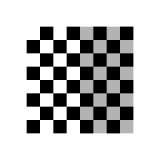
\includegraphics[height=0.8\textwidth]{images/ch_id.pdf}
\end{center}
\end{block}
\end{column}
\begin{column}{0.5\columnwidth}
\begin{block}{Reflection}
\[ \bv{M} =\begin{bmatrix}-1&0&0\\0&1&0\\0&0&1\end{bmatrix} \]
\begin{center}
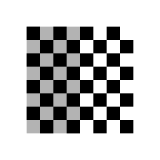
\includegraphics[height=0.8\textwidth]{images/ch_ref.pdf}
\end{center}
\end{block}
\end{column}
\end{columns}
\end{frame}

\begin{frame}[label={sec:org064facd}]{Linear transformations : Examples}
\begin{columns}
\begin{column}{0.5\columnwidth}
\begin{block}{Scale}
\[ \bv{M} =\begin{bmatrix}c_{x}=2&0&0\\0&c_{y}=1&0\\0&0&1\end{bmatrix} \]
\begin{center}
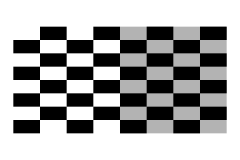
\includegraphics[height=0.8\textwidth]{images/ch_sc.pdf}
\end{center}
\end{block}
\end{column}
\begin{column}{0.5\columnwidth}
\begin{block}{Shear}
\[ \bv{M} =\begin{bmatrix}1&c_{x}=0.5&0\\c_{y}=0&1&0\\0&0&1\end{bmatrix}\]
\begin{center}
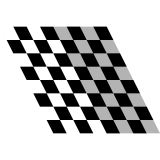
\includegraphics[height=0.8\textwidth]{images/ch_sh.pdf}
\end{center}
\end{block}
\end{column}
\end{columns}
\end{frame}

\begin{frame}[label={sec:org6ca2e18}]{Linear transformations : Examples}
\begin{block}{Rotation}
\begin{center}
\spot<2>{\( \bv{M} =\begin{bmatrix}\cos(\theta )&\sin(\theta )&0\\-\sin(\theta
 )&\cos(\theta )&0\\0&0&1\end{bmatrix} \text{with } \theta = \frac{\pi}{6}\)}
\end{center}

\begin{center}
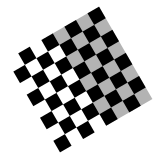
\includegraphics[height=0.5\textwidth]{images/ch_rot.pdf}
\end{center}
\end{block}
\end{frame}
\begin{frame}[label={sec:orgfed4950}]{Rotations (includes reflections)}
\begin{itemize}
\item Generates new unit vectors, fundamentally changing the directions
(eigenvectors) of further transformations
\item Does not scale the entity under consideration ( \(\abs{\lambda} \equiv  1\), more on this later\ldots{})
\end{itemize}
\end{frame}
\begin{frame}[label={sec:org55a71e8}]{Frame rotations in two--dimensions}
Consider rotation in two dimensions:


% 3D axis with spherical coordinates
\tdplotsetmaincoords{0}{0}
\begin{center}
\begin{tikzpicture}[scale=3,tdplot_main_coords]

	% variables
	\def\rvec{0.8}
	\def\thetavec{90}
	\def\phivec{36.86}

	% variables
	\def\alphavec{20}

	% axes
	\coordinate (O) at (0,0,0);
	\draw[thick,->] (0,0,0) -- (1,0,0) node[anchor=north east]{$x$};
	\draw[thick,->] (0,0,0) -- (0,1,0) node[anchor=north west]{$y$};


	% vectors
	\tdplotsetcoord{P}{\rvec}{\thetavec}{\phivec}
	% Draw point at P
	\filldraw [color=metropolisblue](P) circle (0.02) ;
	\draw[-stealth,metropolisblue,thick] (O)  -- (P) node[above right] {$p$};
	\draw[metropolisblue]   (P)  -- (Px) node[below] {$p_x$};
	\draw[metropolisblue]   (P)  -- (Py) node[left] {$p_y$};

	% coordinate axes xdash and ydash
	\tdplotsetcoord{xdash}{1}{90}{\alphavec}
	\tdplotsetcoord{ydash}{1}{90}{\alphavec + 90}
	\draw[->,metropolisorange,dashed] (O)  -- (xdash) node[above right] {$x^{\prime}$};
	\draw[->,metropolisorange,dashed] (O)  -- (ydash) node[above right] {$y^{\prime}$};

	% Points on x and y dash
	\tdplotsetcoord{xdashmeet}{\rvec*cos(\phivec-\alphavec)}{90}{\alphavec}
	\tdplotsetcoord{ydashmeet}{\rvec*sin(\phivec-\alphavec)}{90}{\alphavec + 90}
	\draw[metropolisorange]   (P)  -- (xdashmeet) node[below right] {$p_x^{\prime}$};
	\draw[metropolisorange]   (P)  -- (ydashmeet) node[below left] {$p_y^{\prime}$};

	% arcs
	\tdplotdrawarc[->]{(O)}{0.4}{0}{\alphavec}
	{anchor=west}{$\alpha$}
	% \tdplotsetthetaplanecoords{\phivec}
	% \tdplotdrawarc[->,tdplot_rotated_coords]{(0,0,0)}{0.5}{0}{\thetavec}
	% {anchor=south west}{$\theta$}
\end{tikzpicture}
\end{center}

\[ \begin{bmatrix} x^\prime \\ y^\prime \end{bmatrix}
   = \underbrace{\begin{bmatrix}\cos(\alpha )&\sin(\alpha )\\ -\sin(\alpha
   )&\cos(\alpha )\end{bmatrix}}_{\bv{R}} \begin{bmatrix} x\\ y\end{bmatrix}\]
\note{:B\_note:
Derive this thing in class.}
\end{frame}
\begin{frame}[label={sec:orga43576e}]{Inverse rotations in two--dimensions}
Now consider the same picture, but we want to obtain \([x,y]^T\) from \([
   x^\prime, y^\prime ]^T\) (the other way around).

\begin{itemize}
\item Physically, this is just a rotation of \(- \alpha\) counter-clockwise (or
\(\alpha\) clockwise). That means
\end{itemize}
\[ \begin{bmatrix} x\\ y\end{bmatrix}
   = \begin{bmatrix}\cos(\alpha )& -\sin(\alpha )\\ \sin(\alpha
   )& \cos(\alpha )\end{bmatrix}  \begin{bmatrix} x^\prime \\ y^\prime
   \end{bmatrix} \]
\begin{itemize}
\item Mathematically, if \(\gv{x}^\prime= \bv{R} \gv{x}\), then we know \(\gv{x}= \bv{R}^{-1} \gv{x}^\prime\), provided \(\bv{R}^{-1}\) exists
(which does).
\item Then notice that
\end{itemize}
\[ \bv{R}^{-1} = \begin{bmatrix}\cos(\alpha )& -\sin(\alpha )\\ \sin(\alpha
   )& \cos(\alpha )\end{bmatrix}  = \bv{R}^T ! \]
\begin{itemize}
\item We will see later why holds for \alert{all} rotation matrices\ldots{}
\end{itemize}
\end{frame}
\begin{frame}[label={sec:org0a8b6f5}]{Frame rotations in three--dimensions}
\begin{figure}[htbp]
\centering
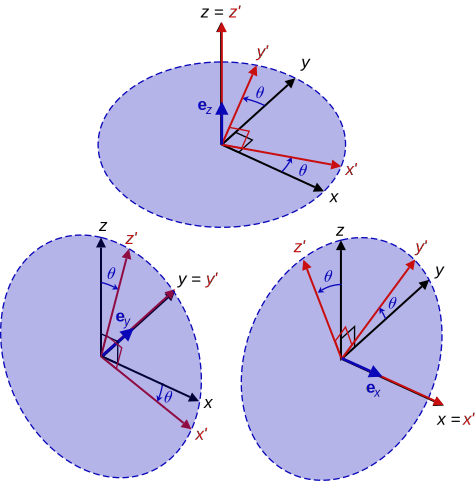
\includegraphics[width=0.45\textwidth]{images/cartesian_rot_3D.pdf}
\caption{Rotation in three dimensions, Wikimedia CC1.0}
\end{figure}
is a natural extension of 2D results\ldots{}
\end{frame}
\begin{frame}[label={sec:org75d4572}]{Beware!}
\begin{block}{Be wary about alias (passive) or alibi (active) transformations}
\end{block}
\begin{columns}
\begin{column}{0.55\columnwidth}
\begin{definition}[Alias transformations]
Involves rotation of the coordinate system or frame
(change in basis)
\end{definition}
\begin{definition}[Alibi transformations]
Involves rotation of the entities within the same
frame (change in entity)
\end{definition}
\end{column}
\begin{column}{0.5\columnwidth}
\begin{figure}[htbp]
\centering
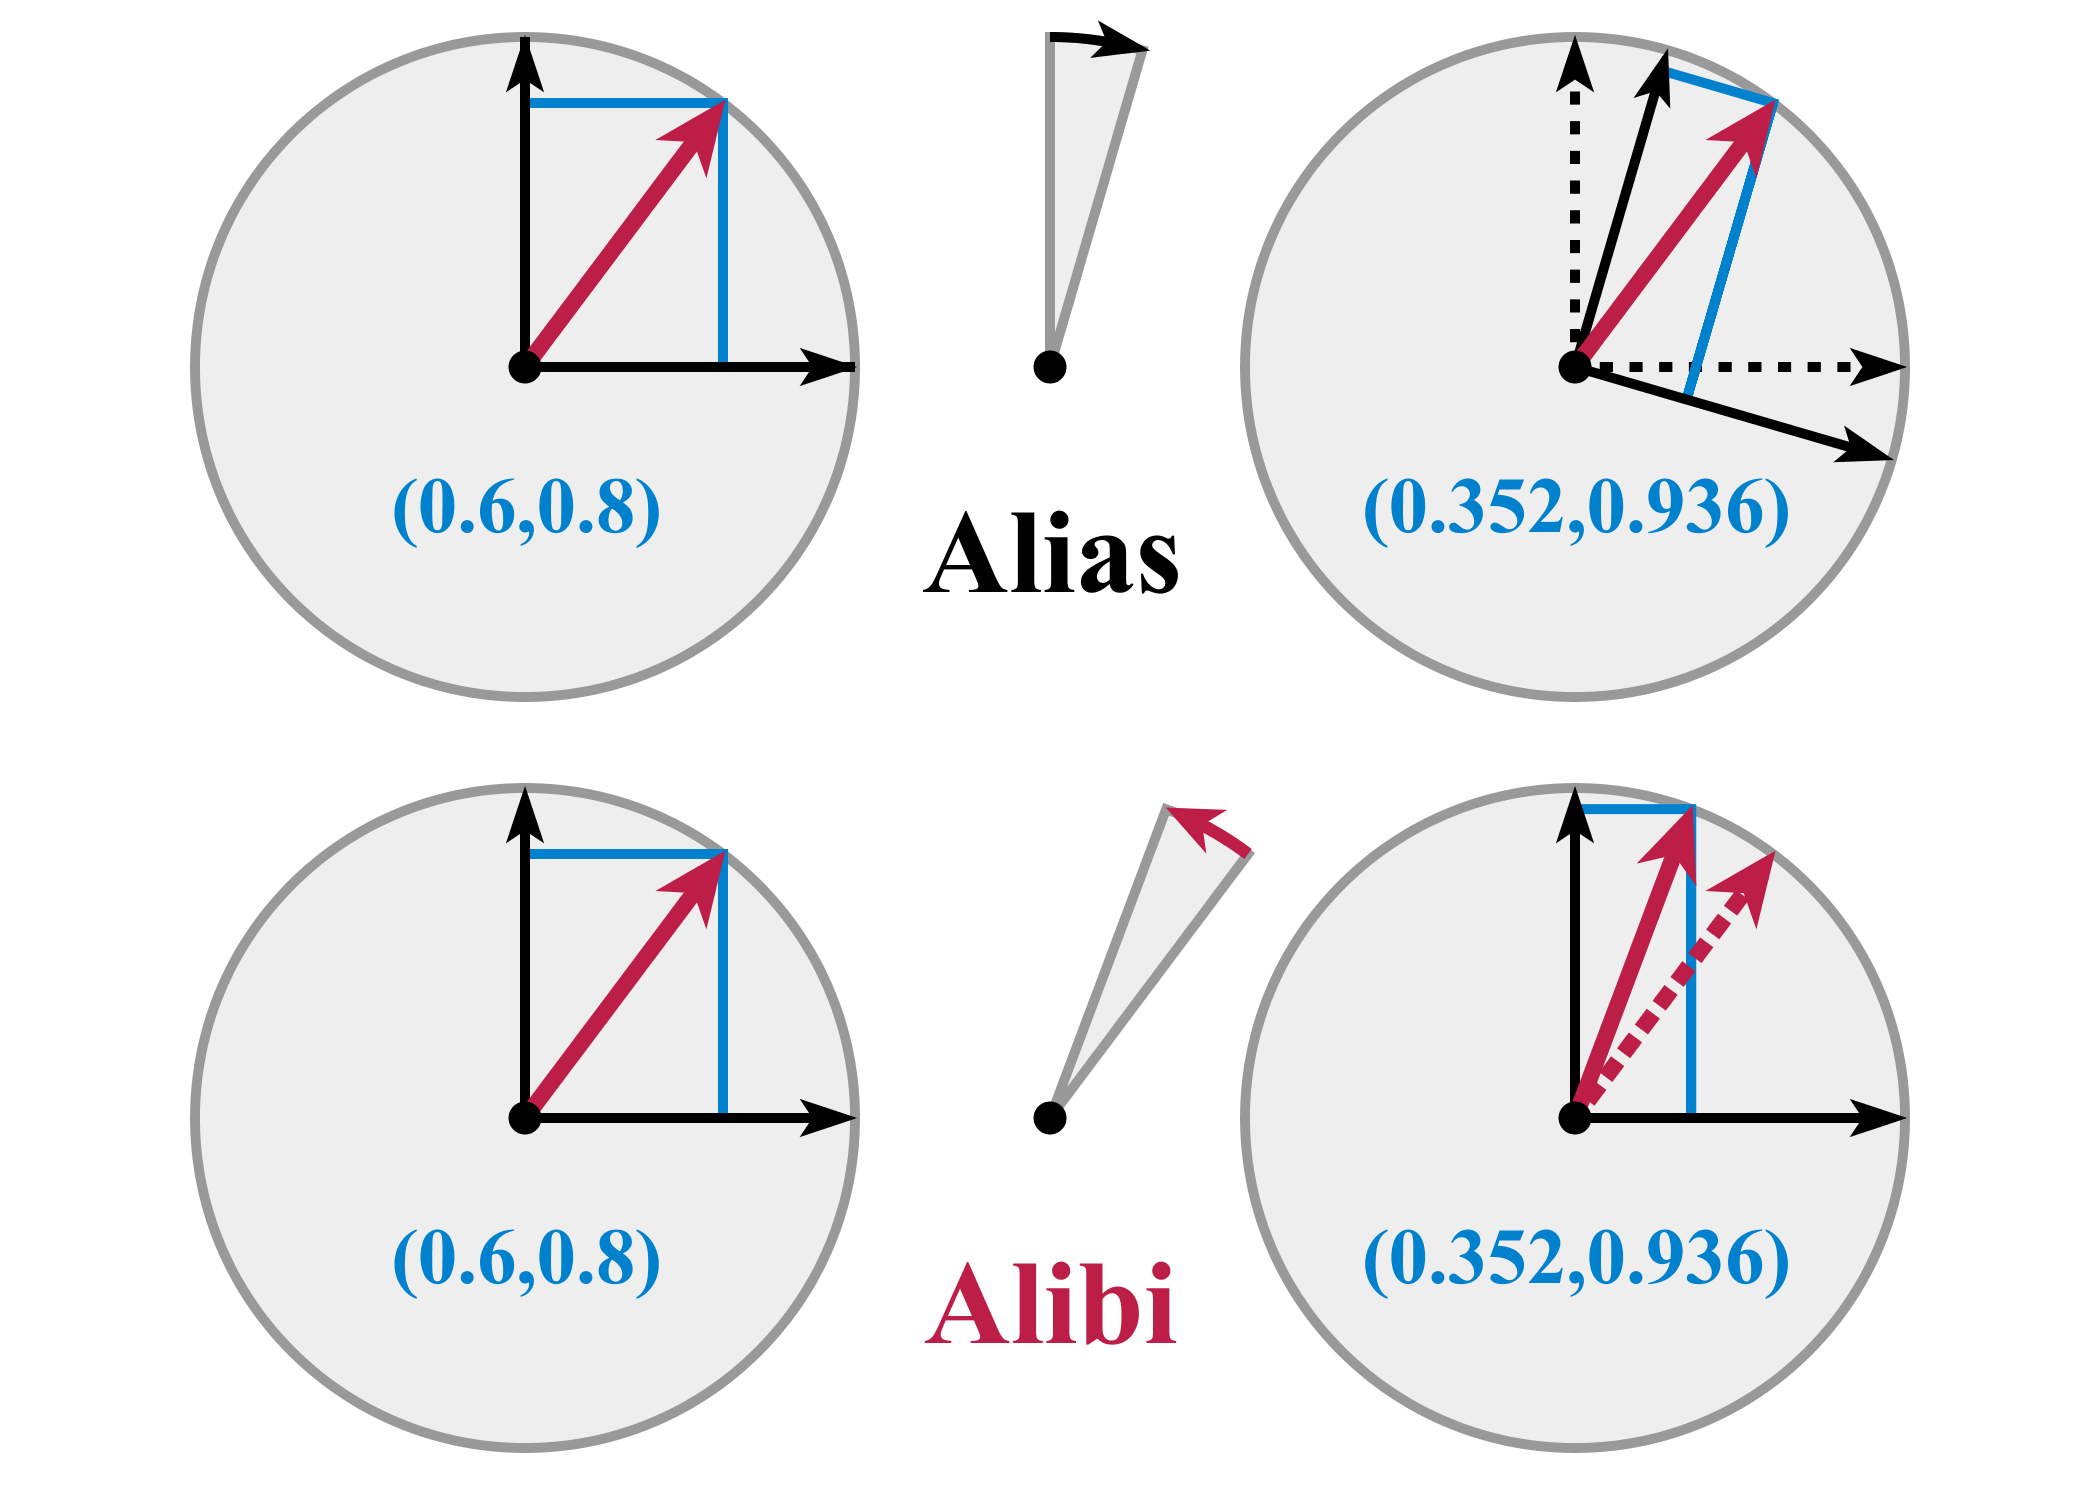
\includegraphics[width=1.00\textwidth]{images/alias_alibi.png}
\caption{Alias-Alibi transformations, Wikimedia CC3.0}
\end{figure}
\end{column}
\end{columns}
Both are equally valid ways of representing rotations---in this class
however, we focus on alias transformations.
\note{:B\_note:
\begin{itemize}
\item Affirm that the entity does not matter. Show this for a vector or a point.
Beauty of affine transformations.
\item To change the formulas for passive rotations (or find reverse active
rotation), transpose the matrices (then each matrix transforms the initial
coordinates of a vector remaining fixed to the coordinates of the same
vector measured in the rotated reference system; same rotation axis, same
angles, but now the coordinate system rotates, rather than the vector).
\end{itemize}}
\end{frame}
\begin{frame}[label={sec:orgcae70fc}]{Difference in perspectives\footnote{\href{https://iopscience.iop.org/book/978-0-7503-1454-1}{Rotation, Reflection, and Frame Changes---Orthogonal tensors in computational engineering mechanics, RM Brannon, IOP Publishing 2018}}}
\begin{quotation} %% :B\_quotation:
`` Analyzing rotation demands awareness of your desired perspective. You can rotate an object, while you stay still, or you can keep the object
fixed while you rotate yourself. It is important to be aware of which of these
perspectives applies for your problem of interest. The distinction between
these fundamentally different transformations goes beyond one being the
same as the other with an opposite rotation angle. ''
\end{quotation}
\end{frame}
\begin{frame}[label={sec:org8c24a79}]{Frame rotation as a change in basis}
\begin{block}{More concretely}
If \(\mathcal{B}\) and \(\mathcal{B}^\prime\) are two (different) bases
\(\in \mathbb{R}^n\)
\begin{itemize}
\item Alibi : Change in entity \([\gv{p}]_{\mathcal{B}} \to
      [\gv{p}^\prime]_{\mathcal{B}}\) given by
\end{itemize}
\[ [\gv{p}^\prime]_{\mathcal{B}} = [\bv{M}]_{\mathcal{B} \to \mathcal{B}}
  [\gv{p}]_{\mathcal{B}} \]
\begin{itemize}
\item Alias : Change in basis \([\gv{p}]_{\mathcal{B}} \to
      [\gv{p}]_{\mathcal{B}^\prime}\)
\end{itemize}
\[ [\gv{p}]_{\mathcal{B}^\prime} = [\bv{M}]_{\mathcal{B} \to \mathcal{B}^\prime}
  [\gv{p}]_{\mathcal{B}} \]
\begin{itemize}
\item In our soft filament framework, \(\mathcal{B}^\prime \equiv \mathcal{L}\) and  \(\mathcal{B} \equiv\) lab frame. \(\bv{Q}\) is then the
basis transformation matrix (corresponding to pure rotation of the
orthonormal bases)
\end{itemize}
\end{block}
\end{frame}
\begin{frame}[label={sec:org227e977}]{Frame rotation---example}
\begin{columns}
\begin{column}{0.5\columnwidth}
\tdplotsetmaincoords{60}{100}
\begin{center}
 \begin{tikzpicture}[scale=2, tdplot_main_coords]
 \draw[thick,->, color=scarlet] (0,0,0) -- (1,0,0) node[anchor=north east]{$x$};
 \draw[thick,->, color=shamrockgreen] (0,0,0) -- (0,1,0) node[anchor=north west]{$y$};
 \draw[thick,->, color=royalblue] (0,0,0) -- (0,0,1) node[anchor=south]{$z$};
 \end{tikzpicture}
\end{center}
\end{column}
\begin{column}{0.5\columnwidth}
\tdplotsetmaincoords{60}{100}
\begin{center}
 \begin{tikzpicture}[scale=2, tdplot_main_coords]
 \draw[dashed,->,line width= 1.1pt] (0,0,0) -- (1,0,0) node[anchor=north east]{$x$};
 \draw[dashed,->,line width= 1.1pt] (0,0,0) -- (0,1,0) node[anchor=north west]{$y$};
 \draw[dashed,->,line width= 1.1pt] (0,0,0) -- (0,0,1) node[anchor=south west]{$z$};

 \coordinate (Shift) at (0,0,0);
 \tdplotsetrotatedcoords{0}{0}{90}
 \tdplotsetrotatedcoordsorigin{(Shift)}

 \draw[thick,color=scarlet,tdplot_rotated_coords,->] (0,0,0)
 -- (1,0,0) node[anchor=south east]{$x’$};
 \draw[thick,color=shamrockgreen,tdplot_rotated_coords,->] (0,0,0)
 -- (0,1,0) node[anchor=west]{$y’$};
 \draw[thick,color=royalblue,tdplot_rotated_coords,->] (0,0,0)
 -- (0,0,1) node[anchor=south east]{$z’$};
 \end{tikzpicture}
\end{center}
\end{column}
\end{columns}
\begin{itemize}
\item Represent \((x-y-z)\) axis with a basis \(\mathcal{E}\) of unit vectors \(\hat{\gv{e}_1}, \hat{\gv{e}_2}, \hat{\gv{e}_3}\)
\item Represent \((x'-y'-z')\) axis with a basis \(\mathcal{D}\) of unit vectors \(\hat{\gv{d}_1}, \hat{\gv{d}_2}, \hat{\gv{d}_3}\)
\item \(\mathcal{E} \to \mathcal{D}\)?
\item Note : rotation of \(\ang{90}\) about an invariant \(z' = z\) axis
\end{itemize}
\end{frame}
\begin{frame}[label={sec:orgfebea24}]{Frame rotation---example contd.}
\[ {\begin{bmatrix} x^\prime \\ y^\prime \\ z^\prime\end{bmatrix}} =
  \spot{[\bv{M}]_{\mathcal{E} \to \mathcal{D}}}
  {\begin{bmatrix} x \\ y \\ z \end{bmatrix}}
  \]
\begin{itemize}
\item We begin by noticing that \(\begin{bmatrix} x^\prime , y^\prime , z^\prime
     \end{bmatrix} = \begin{bmatrix} y , -x , z \end{bmatrix}\) (from figure). Then
\end{itemize}
\[ {\begin{bmatrix} x^\prime \\ y^\prime \\ z^\prime\end{bmatrix}} =
  {\begin{bmatrix} 0 & 1 & 0 \\ -1 & 0 & 0 \\ 0 & 0 & 1 \end{bmatrix}}
  {\begin{bmatrix} x \\ y \\ z \end{bmatrix}}
  \]
\[\Rightarrow {\begin{bmatrix} x^\prime \\ y^\prime \\ z^\prime\end{bmatrix}} =
  {\begin{bmatrix} \cos(\ang{90}) & \sin(\ang{90}) & 0 \\ -\sin(\ang{90}) &
  \cos(\ang{90}) & 0 \\ 0 & 0 & 1 \end{bmatrix}}
  {\begin{bmatrix} x \\ y \\ z \end{bmatrix}}
  \]
\end{frame}
\begin{frame}[label={sec:org991b3fb}]{Generalizing frame rotations as a basis change}
\begin{itemize}
\item But also notice with the given bases that
\end{itemize}
\[{\begin{bmatrix} x^\prime \\ y^\prime \\ z^\prime\end{bmatrix}_{\mathcal{D}}} =
  \spot<2>{
  \underbrace{\begin{bmatrix}
  \hat{\gv{d}}_1 \cdot \hat{\gv{e}}_1 & \hat{\gv{d}}_1 \cdot
  \hat{\gv{e}}_2 & \hat{\gv{d}}_1 \cdot \hat{\gv{e}}_3 \\
  \hat{\gv{d}}_2 \cdot \hat{\gv{e}}_1 & \hat{\gv{d}}_2 \cdot
  \hat{\gv{e}}_2 & \hat{\gv{d}}_2 \cdot \hat{\gv{e}}_3 \\
  \hat{\gv{d}}_3 \cdot \hat{\gv{e}}_1 & \hat{\gv{d}}_3 \cdot
  \hat{\gv{e}}_2 & \hat{\gv{d}}_3 \cdot \hat{\gv{e}}_3
  \end{bmatrix}}_{[\bv{M}]_{\mathcal{E} \to \mathcal{D}}, \text{ independent of
  } \mathbf{x}}
  }
  {\begin{bmatrix} x \\ y \\ z \end{bmatrix}_{\mathcal{E}}}
  \]
\begin{block}<2->{Soft filament framework}
\begin{itemize}
\item Describe lab frame, \(\mathcal{E}\), by natural bases \(\hat{i}, \hat{j}, \hat{k}\).
\item Describe material (Lagrangian) frame, \(\mathcal{D}\), by orthonormal
vectors \(\hat{\gv{d}_1}, \hat{\gv{d}_2}, \hat{\gv{d}_3}\) (coordinates wrt
natural bases). Then
\end{itemize}
\[{\begin{bmatrix} x_{\mathcal{L}} \\ y_{\mathcal{L}} \\ z_{\mathcal{L}} \end{bmatrix}_{\mathcal{D}}} =
	 \underbrace{\begin{bmatrix}
	 \mbox{------}~\hat{\gv{d}}_1~\mbox{------} \\
	 \mbox{------}~\hat{\gv{d}}_2~\mbox{------} \\
	 \mbox{------}~\hat{\gv{d}}_3~\mbox{------} \\
	 \end{bmatrix}}_{\bv{Q}}
	 {\begin{bmatrix} x \\ y \\ z \end{bmatrix}_{\mathcal{E}}}
   \]
\end{block}
\note{:B\_note:
\begin{itemize}
\item Derive the \(\gv{d} \cdot \gv{e}\) relations in class.
\end{itemize}}
\end{frame}
\begin{frame}[label={sec:org1903ed5}]{Generalizing frame rotations as a basis change}
 Taking it one step further we arrive at the conclusion,
\[
	\underbrace{\begin{bmatrix}
	\mbox{|} & \mbox{|}& \mbox{|}\\
	\hat{\gv{d}_1} & \hat{\gv{d}_2} & \hat{\gv{d}_3} \\
	\mbox{|} & \mbox{|}& \mbox{|}\\
	\end{bmatrix}}_{\bv{Q}^{-1} = \bv{Q}^T}
	{\begin{bmatrix} x_{\mathcal{L}} \\ y_{\mathcal{L}} \\ z_{\mathcal{L}}
	\end{bmatrix}}
	=
	{\begin{bmatrix}1 & 0 & 0 \\ 0 & 1 & 0 \\0 & 0& 1\end{bmatrix}}
	{\begin{bmatrix} x \\ y \\ z \end{bmatrix}}
  \]

\[
  \Rightarrow x_{\mathcal{L}}\hat{\gv{d}_1} + y_{\mathcal{L}}\hat{\gv{d}_2} +
  z_{\mathcal{L}}\hat{\gv{d}_3} = x\hat{i} + y\hat{j} + z\hat{k} = \gv{x} !
  \]
\note{:B\_note:
\begin{itemize}
\item Again iterate that this is a passive (alias) transformation and so this is
the expected result.
\end{itemize}}
\end{frame}
\begin{frame}[label={sec:org12f3010}]{Implementation of rotation as bases change}
\begin{itemize}
\item We have seen that the action of frame rotation matrices correspond to a
bases change operation
\item Let's implement these operations in our framework
\[ R_{x}(\theta)={\begin{bmatrix}1&0&0\\0&\cos \theta &\sin \theta
     \\0&-\sin \theta &\cos \theta \\\end{bmatrix}}\]

\[ R_{y}(\theta)={\begin{bmatrix}\cos \theta & 0 & -\sin \theta\\
	 0&1&0 \\ \sin\theta & 0 & \cos \theta \\\end{bmatrix}} \]

\[R_{z}(\theta)={\begin{bmatrix}\cos \theta &\sin \theta &0\\-\sin
	 \theta &\cos\theta &0\\0&0&1\\\end{bmatrix}} \]
\item \alert{ACTIVITY}
\end{itemize}
\end{frame}
\begin{frame}[label={sec:orgc5d508b}]{But what about arbitrary rotations?}
\begin{itemize}
\item Rotations about arbitrary axes with arbitrary angles?
\end{itemize}
\begin{columns}
\begin{column}{0.6\columnwidth}
\begin{itemize}
\item Can we do compositions?
\begin{itemize}
\item \alert{Yes}, but not that intutive (means of rotation, intrinsic/extrinsic)
\item Not commutative (order matters) usually
\end{itemize}
\end{itemize}
\end{column}
\begin{column}{0.3\columnwidth}
\begin{center}
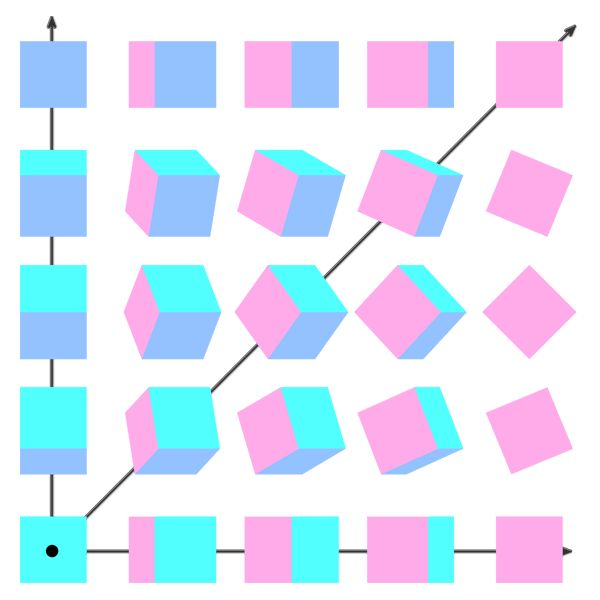
\includegraphics[width=0.80\textwidth]{images/rotated_cube.jpeg}
\end{center}
\end{column}
\end{columns}
\begin{itemize}
\item Becomes even more complicated when we have frames depending on one another
\begin{itemize}
\item But not a bad idea---robotics\footnote{\href{https://www.mecademic.com/resources/Euler-angles/Euler-angles}{Mecademic Euler rotations}}
\end{itemize}
\item \alert{Idea}: If we know the linear bases transformation, we don't need to worry
about compositions etc.
\end{itemize}
\note{:B\_note:
\begin{itemize}
\item Mention that some means of rotation like quarternions are better suited,
but require more math and understanding.
\item Mention Euler axis angle, euler roataions, quarternions
\end{itemize}}
\end{frame}
\begin{frame}[label={sec:orgd186306}]{Let's reconsider what we know}
\begin{itemize}
\item We know why \(\gv{x}_{\mathcal{L}} = \bv{Q}\gv{x}\)
\item We then need the \alert{action} of \(\bv{Q}\) on \(\gv{x}\)
\item But\ldots{}
\begin{itemize}
\item Do we know \(\bv{Q}\) ?
\begin{itemize}
\item We need the basis \(\hat{\gv{d}}_j\)
\end{itemize}
\item Do we know \(\hat{\gv{d}}_j\)?
\begin{itemize}
\item \alert{No}
\end{itemize}
\end{itemize}
\item We seek ways to obtain this basis \(\gv{d}\) and hence \(\bv{Q}\).
\item We will see that we require some properties on \(\gv{d}\) to make \(\bv{Q}\) effect a rotation.
\end{itemize}
\end{frame}
\begin{frame}[label={sec:org72dd77f}]{Obtaining \(\gv{d}, \bv{Q}\) : Properties}
\[\bv{Q} =
	 {\begin{bmatrix}
	 \mbox{------}~\hat{\gv{d}}_1~\mbox{------} \\
	 \mbox{------}~\hat{\gv{d}}_2~\mbox{------} \\
	 \mbox{------}~\hat{\gv{d}}_3~\mbox{------} \\
	 \end{bmatrix}}
   \]
\begin{columns}
\begin{column}{0.47\columnwidth}
\begin{block}{\(\bv{Q}\)}
\begin{itemize}
\item Rows are unit vectors
\item Real, orthogonal matrix ( \(\bv{Q^T}\bv{Q} = \bv{Q}\bv{Q^T} = \bv{I}\) )
\item Eigenvalues are \(\lambda = {1, e^{\pm j \theta}}\)
\item Determinant \(= \prod_{i} \lambda_i = 1\)
\end{itemize}
\end{block}
\end{column}
\begin{column}{0.50\columnwidth}
\begin{block}{\(\hat{\gv{d}}\)}
\begin{itemize}
\item \(\norm{\hat{\gv{d}_1}} = \norm{\hat{\gv{d}_2}} = 1\)
\item \(\hat{\gv{d}_1} \cdot \hat{\gv{d}_2} = 0\)
\item \(\hat{\gv{d}_1} \times \hat{\gv{d}_2} = \hat{\gv{d}_3}\)
\item \(\therefore\) They form an orthonormal basis
\end{itemize}
\end{block}
\end{column}
\end{columns}
\note{:B\_note:
\begin{itemize}
\item Motivate orthogonality by saying that the natural bases is orthogonal,
and so we want to preserve this in rotation (all axes rotates equally).
This also makes R\^{}-1 = R\^{}T
\item By Gram-Schmidt theorem, we can always find an orthonormal bases given a
span of vectors
\item Euler's rotation theorem: Express any roation as a single rotation about
an axis. Eigenvalues represent this. 1--> rotation axes. 2,3 are
orthogonal axes that simply has a rotation.
\item Motivate determinant by volume. It tells expansino of a volume: 1 means
volume is preserved. Formulae for parallelopiped : \(u \cdot (v \times w)\). They are symmetric relations.
\end{itemize}}
\end{frame}
\begin{frame}[label={sec:org8fac1e7}]{Obtaining \(\gv{d}, \bv{Q}\) : Options\footnote{Wikimedia, CC3.0 license}}
\begin{columns}
\begin{column}{0.6\columnwidth}
\begin{itemize}
\item We only need the \alert{action} of \(\bv{Q}\) on \(\gv{x}\)
\item Some means/formalisms to achieve these are
\begin{itemize}
\item Rotation matrices (gives \(\bv{Q}\) explicitly )
\item \(\spot<2>{\text{Euler axes and angle } \gv{r} = \theta \hat{\gv{e}} }\)
\item Euler rotations (precession, nutation, rotation)
\item Quaternions (\(w, \gv{r}\))
\end{itemize}
\item (dis)Advantages are spread equally, although some are more equal than the others*
\end{itemize}
\end{column}
\begin{column}{0.4\columnwidth}
\begin{figure}[htbp]
\centering
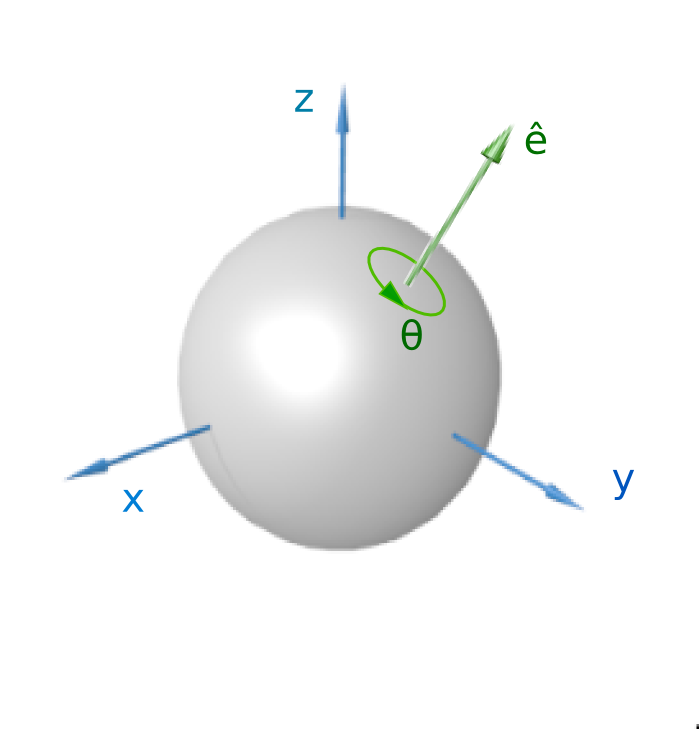
\includegraphics[width=0.45\textwidth]{images/euler_aa.png}
\caption{Euler axis-angle}
\end{figure}
\begin{figure}[htbp]
\centering
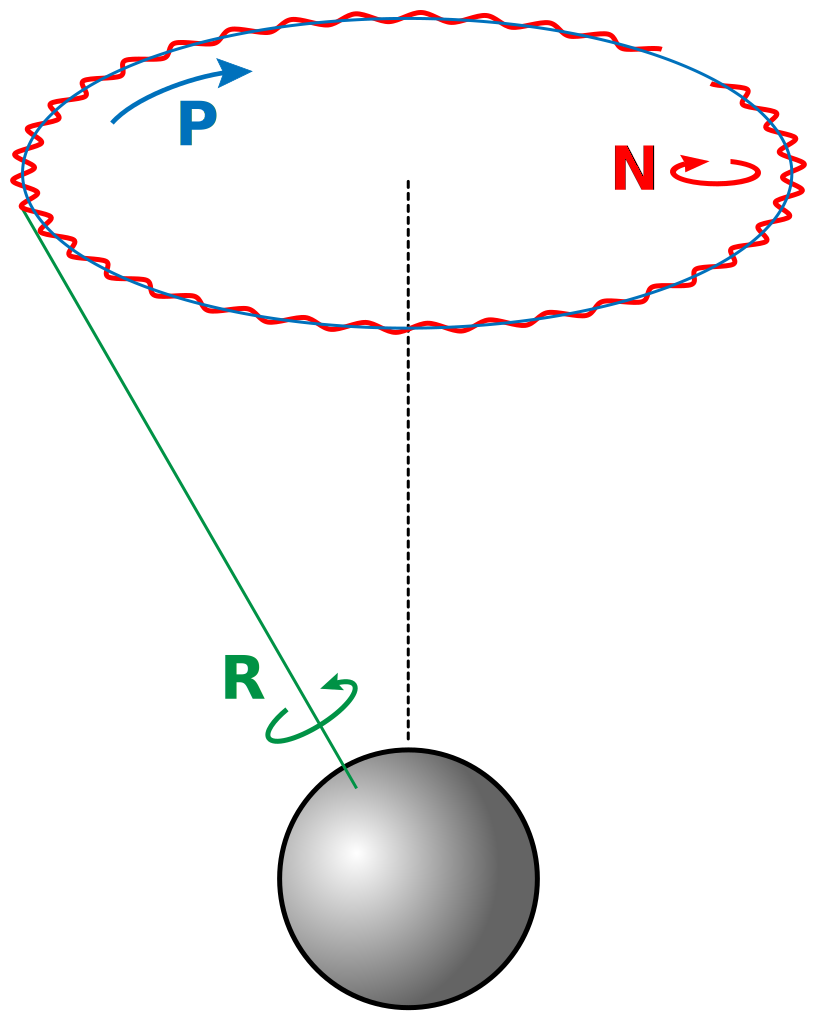
\includegraphics[width=0.45\textwidth]{images/euler_rot.pdf}
\caption{Euler rotations}
\end{figure}
\end{column}
\end{columns}
\end{frame}

\begin{frame}[label={sec:org52a80d1}]{Rotations about fixed axis : Euler axis-angle}
\begin{block}{Single rotation about an axis---\(\hat{\gv{e}}\) vector}
\begin{itemize}
\item Axis : unit vector which remains unchanged by the rotation
\item Note : Only two dofs, by normality condition
\item Unique, for any given rotation, except for the sign
\end{itemize}
\end{block}
\begin{block}{Rotation through scalar \(\theta\)}
\begin{itemize}
\item Unique, sign determined by axis \(\hat{\gv{e}}\)
\end{itemize}
\end{block}
\begin{columns}
\begin{column}{0.6\columnwidth}
\begin{block}{\(\hat{\gv{r}} = \theta \hat{\gv{e}}\)}
\begin{itemize}
\item Called \emph{Rotation vector} or \emph{Euler vector}
\end{itemize}
\end{block}
\end{column}
\begin{column}{0.3\columnwidth}
\begin{figure}[htbp]
\centering
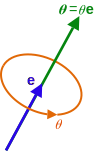
\includegraphics[width=0.45\textwidth]{images/euler_axis.pdf}
\caption{Euler axis-angle}
\end{figure}
\end{column}
\end{columns}
\end{frame}
\begin{frame}[label={sec:orgf520f10}]{Rotations about fixed axis : Euler axis-angle}
\begin{block}{Advantages}
\begin{itemize}
\item Easy to understand/code up
\item Convenient while dealing with rigid body motions
\item Conversion to rotation matrices straightforward (and is so for all other
representations as well)
\end{itemize}
\end{block}
\begin{block}{Disadvantages}
\begin{itemize}
\item Combining successive rotations not straightforward (and breaks vector addition)
\item Corner cases when dealing with \(\theta = 0\) and signs of \(\hat{\gv{e}}\)
\end{itemize}
\end{block}
\end{frame}
\begin{frame}[label={sec:org49088fb}]{Rotation using Euler angles : Rodrigues formula}
\begin{block}{Rodrigues formula}
\begin{itemize}
\item Named after \href{https://en.wikipedia.org/wiki/Olinde\_Rodrigues}{Olinde Rodrigues}
\item Is an efficient algorithm to rotate a vector in space, given \(\theta\)
and \(\hat{\gv{e}}\).
\item Gives the exponential map that effects a transformation from the
axis-angle representation (our case!) to rotation matrices
\item Basically gives us \(\bv{Q}\) given \(\theta \hat{\gv{e}}\).
\end{itemize}
\[ \mathbf {R} =\mathbf {I} +(\sin \theta )\mathbf {K} +(1-\cos \theta )\mathbf {K} ^{2} \]
where \(\mathbf{K}\) is the cross product matrix, discussed last class \(\mathbf{K}\gv{v} = \hat{\gv{e}} \times \gv{v}\)
\end{block}
\end{frame}
\begin{frame}[label={sec:org4c4fa66}]{Rotation matrix from Rodrigues formula : structure and intuition}
 \[ \mathbf {R} =\mathbf {I} +(\sin \theta )\mathbf {K} +(1-\cos \theta )\mathbf {K} ^{2} \]
We need \(\bv{R}\) above to satisfy properties of a rotation matrix. Let's verify:
\begin{itemize}
\item \(\bv{R}(0) = \bv{I}\)
\item \(\bv{R}(\theta)\bv{R}(\phi) = \bv{R}(\theta+\phi)\)
\item \(\bv{R}\bv{R}^T = \bv{R}^T\bv{R} = \bv{I}\)
\end{itemize}
We note that this operator always exists and is unique for given axis-angle
(hence its form).
\note{:B\_note:
\begin{itemize}
\item Use k\^{}4 = -k\^{}2 in the rr\^{}T thing
\item Use k\^{}T = -k.
\end{itemize}}
\end{frame}
\begin{frame}[label={sec:org13b137e},fragile]{Simplification using sympy}
 \begin{minted}[]{python}
import sympy as sp
from sympy.simplify.fu import TR8, TR9, TR10i
x, y, k = sp.symbols('x y k')
expr_x = 1 + sp.sin(x)*k + (1-sp.cos(x))*k**2
expr_y = 1 + sp.sin(y)*k + (1-sp.cos(y))*k**2
expr_n = sp.fu(expr_x * expr_y,
             measure=lambda x: -x.count_ops())
# expr = TR8(expr_x * expr_y)
# print(TR9(expr))
print(expr_n)
\end{minted}

\begin{verbatim}
k**4*cos(x)*cos(y) - 2*k**4*cos(x/2 - y/2)*cos(x/2 + y/2) + k**4 + 2*k**3*sin(x/2 + y/2)*cos(x/2 - y/2) - k**3*sin(x + y) + k**2*sin(x)*sin(y) - 2*k**2*cos(x/2 - y/2)*cos(x/2 + y/2) + 2*k**2 + 2*k*sin(x/2 + y/2)*cos(x/2 - y/2) + 1
\end{verbatim}
\end{frame}

\begin{frame}[label={sec:org3a282a8}]{Rotation using Euler angles : Rodrigues formula (geometry)}
But where did it come from?
\alert{GEOMETRY} (part I)
\begin{figure}[htbp]
\centering
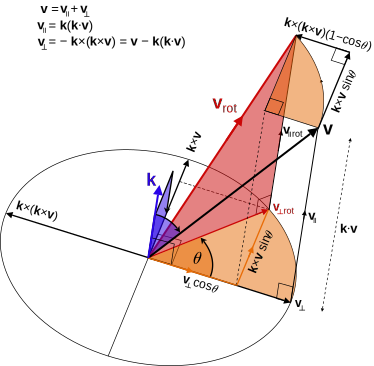
\includegraphics[width=0.45\textwidth]{images/rodrigues.pdf}
\caption{Geometrical construction for deriving the Rodrigues rotation formula}
\end{figure}
\[ \gv{v}_{\mathrm {rot} } =\cos \theta \,\gv{v} +(1-\cos \theta
)(\gv {k} \cdot \gv {v} )\gv {k} +\sin \theta \,\gv {k} \times
\gv {v} \]
\end{frame}
\begin{frame}[label={sec:org2bd26ba}]{Rotation using Euler angles : Rodrigues formula (geometry)}
 \alert{GEOMETRY} (part II)
 Given
\[ \gv {v}_{\mathrm {rot} } =\cos \theta \,\gv {v} +(1-\cos \theta
  )(\hat{\gv {k}} \cdot {\gv{v}} ) \hat{\gv{k}} +\sin \theta \,\hat{\gv{k}} \times
  \gv {v} \]

With \(\mathbf{K}\gv{v} = \hat{\gv{k}} \times \gv{v}\), we have \(\mathbf{K}\left(
  \mathbf{K} \gv{v}\right) =  \hat{\gv{k}} \times \hat{\gv{k}} \times \gv{v}
  = (\hat{\gv{k}} \cdot \gv{v}) \hat{\gv{k}} - (\hat{\gv{k}} \cdot \hat{\gv{k}})
  \hat{v}\) (Using vector triple product).

Substitute in the original equation,
\[  \gv{v}_{\mathrm {rot} }=\gv {v} +(\sin \theta )\gv {K} \gv {v}
  +(1-\cos \theta )\gv {K} ^{2}\gv {v} \,,\quad \|\gv {K} \|_{2}=1
  \]

Now factor \(\gv{v}\) from the equation to get \(\gv{v}_{\mathrm {rot} } = \mathbf{R}\gv{v}\)
\end{frame}
\begin{frame}[label={sec:org81d311d}]{Digression: ODEs}
\begin{itemize}
\item To further understand the Rodrigues rotation formula (and how it relates
to solving \(\frac{\partial \bv{d}_j}{\partial t} = \omega \times \bv{d}_j\) ), we digress a bit and deal with ordinary differential equations (and
their solutions)
\item The next lecture also deals with the same issues (time-stepping and
numerical stability) and the fundamentals are the same.
\end{itemize}
\begin{example}<1->[Solve the following ODE]
\[ \frac{dx}{dt} = 2x \]
\end{example}
\begin{alertblock}<2->{We can't!}
\begin{itemize}
\item Uniqueness and existence?
\item Initial conditions?
\end{itemize}
\end{alertblock}
\end{frame}
\begin{frame}[label={sec:org9b3af93}]{Digression: simple ODEs}
\begin{example}[Solve the following ODE]
\[ \frac{dx}{dt} = 2x \quad x(0) = 1 \]
\end{example}
\begin{block}{We can!}
\[ x(t) = e^{2t}\]
\end{block}
\end{frame}
\begin{frame}[label={sec:org650f746}]{Digression: system of simple ODEs}
\begin{example}[Solve the following ODE]
\[ \begin{bmatrix}\dot{x} \\ \dot{y} \end{bmatrix} =
	 \begin{bmatrix} 5 & 0 \\ 0 & 3 \end{bmatrix} \cdot
	 \begin{bmatrix}{x} \\ {y} \end{bmatrix} \quad x(0) = 1, y(0) = 2\]
\end{example}
\begin{block}{We can solve this too}
\[ x(t) = e^{5t} \quad y(t) = 2e^{3t} \]

More importantly,
\[ \gv{x}(t) = e^{\bv{A}t}\gv{x}(0)\]
\end{block}
\note{:B\_note:
\begin{itemize}
\item Explain matrix exponential to these dudes
\end{itemize}}
\end{frame}
\begin{frame}[label={sec:org73fdfb3}]{Digression: changing it up a bit}
\begin{example}[Solve the following ODE]
\[ \begin{bmatrix}\dot{x} \\ \dot{y} \end{bmatrix} =
	 \begin{bmatrix} 0 & 1 \\ -1 & 0 \end{bmatrix} \cdot
	 \begin{bmatrix}{x} \\ {y} \end{bmatrix} \quad x(0) = 1, y(0) = 0\]
\end{example}
\begin{block}<2->{We can solve this too!}
\[ x(t) = cos{t} \quad y(t) = \sin{t} \]
\alert{OR}
\[ x(\theta) = cos{\theta} \quad y(\theta) = \sin{\theta} \]
\end{block}
\begin{alertblock}<3->{Matrix exponential}
We still retain \[ \gv{x}(\theta) = e^{\bv{A}\theta}\gv{x}(0) \]
\end{alertblock}
\note{:B\_note:
\begin{itemize}
\item Use Hamiltonian. That is dy/dx = x/y and then integrate
\end{itemize}}
\end{frame}
\begin{frame}[label={sec:org920acc6}]{Digression: changing it up a bit}
\begin{example}[Solve the following ODE]
\[ \begin{bmatrix}\dot{x} \\ \dot{y} \end{bmatrix} =
	 \begin{bmatrix} 0 & 1 \\ -1 & 0 \end{bmatrix} \cdot
	 \begin{bmatrix}{x} \\ {y} \end{bmatrix} \quad x(0) = 1, y(0) = 0\]
\end{example}
\begin{block}{What changed the solutions from exponentials to trigonometric terms?}
\begin{itemize}
\item The skew-symmetry of the matrix!
\item More importantly, a skew-symmetric matrix has a pair of imaginary
eigenvalues \(\pm j \theta\)
\item We know \(\mathrm{Re}{(e^{j \theta})} = \cos(\theta)\), which is exactly
what we see\ldots{}
\item \alert{IDEA} : Matrix exponentials can also be used to perform rotations!
\item Then, can you connect it back to why \(\frac{\partial \bv{d}_j}{\partial t} = \omega \times \bv{d}_j\) performs a rotation?
\end{itemize}
\end{block}
\end{frame}
\begin{frame}[label={sec:orgd7e1fa8}]{Rotation using Euler angles : Rodrigues formula (algebra)}
With \(\mathbf{K}\gv{v} = \hat{\gv{k}} \times \gv{v}\), we have
\[ \bv{R}=\exp(\theta \bv {K} )=\sum _{k=0}^{\infty }{\frac {(\theta \bv
{K} )^{k}}{k!}}= \bv{I} + \theta \bv {K} + {\frac {1}{2!}}(\theta \bv {K}
)^{2} + {\frac {1}{3!}}(\theta \bv {K} )^{3} + \cdots  \]

Because of skew-symmetry and orthogonality, by Cayley-Hamilton theorem we have, \(\mathbf {K} ^{3}=-\mathbf {K}, \mathbf {K}^{4}=-\mathbf{K}^2,\mathbf
  {K}^{5}=\mathbf{K},\mathbf{K}^{6}=\mathbf{K}^2\).

With this cyclic pattern continuing for \(k \to \infty\), we have
\(\bv{R}=\bv{I}+\left(\theta -{\frac {\theta ^{3}}{3!}}+{\frac {\theta
  ^{5}}{5!}}-\cdots \right)\mathbf{K} +\left({\frac {\theta ^{2}}{2!}}-{\frac
  {\theta ^{4}}{4!}} + {\frac {\theta ^{6}}{6!}}-\cdots \right) \mathbf{K} ^{2}\)

or equivalently

\(\mathbf {R} =\mathbf {I} +(\sin \theta )\mathbf {K} +(1-\cos \theta )\mathbf {K} ^{2}\)
\end{frame}
\begin{frame}[label={sec:org3ebb2ce}]{Rotation : Rodrigues formula implementation}
\begin{itemize}
\item We have seen how the matrix exponential can give rise to rotation.
\item Let's implement this operation in our framework
\end{itemize}
\[ \mathbf {R} =\mathbf {I} +(\sin \theta )\mathbf {K} +(1-\cos \theta )\mathbf {K} ^{2} \]
, \(\bv{K}\) being the now-familiar skew-symmetric matrix having vector elements
\[ \mathbf {K} = \begin{bmatrix}\,\,0&\!-k_{3}&\,\,\,k_{2}\\\,\,\,k_{3}&0&\!-k_{1}\\\!-k_{2}&\,\,k_{1}&\,\,0\end{bmatrix}
   \]
\begin{itemize}
\item \alert{ACTIVITY}
\end{itemize}
\end{frame}
\begin{frame}[label={sec:org516fbc7}]{Rotation : Rodrigues formula IRL}
\begin{itemize}
\item In mechanics, frame rotations are omnipresent
\item One familiar real life example is when an elastic rod experiences a
torsional force
\begin{figure}[htbp]
\centering
\includegraphics[width=0.45\textwidth]{images/twisted_bar.png}
\caption{Euler rotations}
\end{figure}
\item Let's see this in our framework too\ldots{}
\item \alert{DEMO}
\item It was possible to code the frames up that way (linearly), because of the
spatial rate of change of the frame angle.
\item \alert{Curvature}
\end{itemize}
\end{frame}
\begin{frame}[label={sec:orgcc641f6}]{Rodrigues formula : The inverse operator}
\begin{block}{What about the inverse operation?}
Given the rotation matrix \(\bv{R}\)
\begin{itemize}
\item Identify \(\theta\)
\item Identify \(\hat{\gv{e}}\), the axis
\end{itemize}
\end{block}
\begin{block}{Is it useful?}
Very. Especially when:
\begin{itemize}
\item computing the angle by which two frames differ (especially in graphics)
\item there are governing equations that need differences of, rather than
angles themselves (invariance principles)
\end{itemize}
\end{block}
\begin{block}{How to do it?}
Using the \alert{matrix logarithm} \(\log(\cdot)\) operator, which relies on properties of the
rotation matrix\ldots{}
\end{block}
\end{frame}
\begin{frame}[label={sec:orgf7e2eb4}]{Rodrigues formula : The logarithm operator}
\begin{block}{Formula for \(\theta\)}
\[ \theta = \arccos\left( \frac{\text{Tr}(\mathbf{R}) - 1}{2}\right) \]
Why?
\begin{itemize}
\item trace of a matrix is invariant and \(= \sum \lambda_i\).
\item For a rotation matrix, \(\lambda = {1, e^{\pm j \theta}}\)
\item \(\therefore\) \(\sum \lambda_i = 1 + 2 \cos(\theta)\)
\end{itemize}
\end{block}
\begin{block}{Once \(\theta\) is known, we can find \(\hat{\gv{e}}\)\ldots{}}
\end{block}
\end{frame}
\begin{frame}[label={sec:org3affdd5}]{Rodrigues formula : The logarithm operator}
\begin{block}{Finding \(\hat{\gv{e}}\)\ldots{}}
 Use properties of \(\mathbf{R}\)
\[ \mathbf {R} =\mathbf {I} +(\sin \theta )\mathbf {K} +(1-\cos \theta )\mathbf {K} ^{2} \]
Transposing, using \(\mathbf{K}^T = -\mathbf{K}\) and \((\mathbf{K}^2)^{T} = \mathbf{K}^2\)
\[ \mathbf {R}^T =\mathbf {I} - (\sin \theta )\mathbf {K} +(1-\cos \theta )\mathbf {K} ^{2} \]
Subtracting both the equations,
\[ \mathbf{K} = \left( \frac{\mathbf {R} - \mathbf {R}^T}{2 \sin \theta} \right) \]
\end{block}
\end{frame}
\begin{frame}[label={sec:orge4e58c7}]{Summary}
In this lecture, we
\begin{itemize}
\item understood basic linear/affine transformations relevant in mechanics
\item investigated rotations, and interpreted them as basis-change
transformations
\item saw properties on \(\gv{d}, \bv{Q}\) that linked them back to rotation
\item learnt (+ implemented) a couple (more importantly, the Rodrigues formula)
of ways to rotate basis frames
\end{itemize}
\end{frame}
\begin{frame}[label={sec:org5a852d4}]{Temporal/Spatial rates of change}
What about temporal/spatial changes in rotation? i.e. given a frame, and
given its \emph{change}, how do we predict nearby frames (in time and space)?

\alert{DEMO}
\end{frame}
\end{document}
